\documentclass{summarysheet}

\begin{document}


\maketitle{12}{Nuclear Physics}

\begin{multicols}{2}

\begin{topicbox}{The Nucleus}

\begin{multicols}{2}
\noindent The nucleus of an atom consists of protons and neutrons, which are referred to as \emph{nucleons}.
\begin{itemize}
\item The proton has a charge $+e$ and mass 1.00728 u $=$ 938.27 MeV/$c^2$.  The number of protons in a nucleus is $Z$.
\item The neutron is neutral and has a mass 1.00866 u $=$ 939.56 MeV/$c^2$.  The number of neutrons in a nucleus is $N$.
\item The mass number of a nucleus is the total number of nucleons, $A = Z + N$.  Atoms with different values of $N$ are called \emph{isotopes}.
\end{itemize}

\vspace{0.2in}

\begin{center}
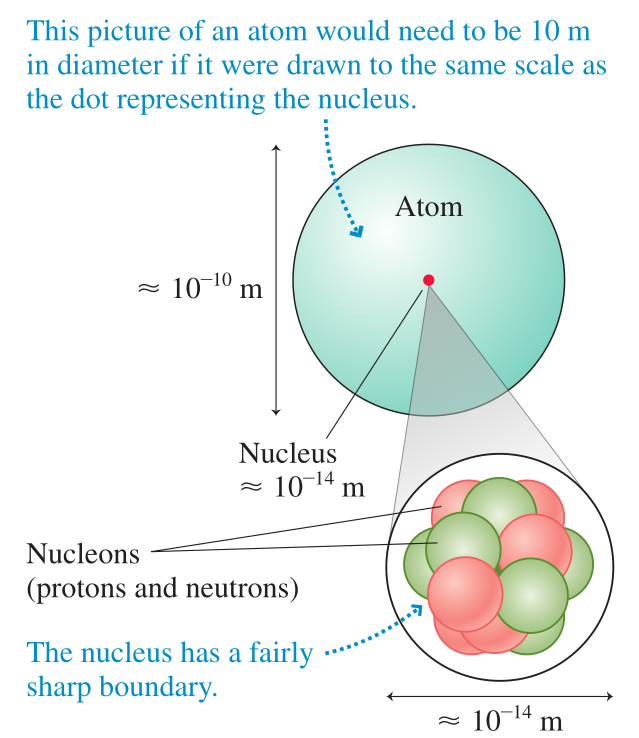
\includegraphics[scale=0.19]{fig_nucleus.png}
\end{center}

\end{multicols}

The radius of a nucleus with mass number $A$ is
\[
R = r_0 A^{1/3},
\]
where $r_0 = 1.2$ fm.  The volume of the nucleus is therefore proportional to $A$.  This implies that nucleons are \emph{incompressible}, tightly packed within the nucleus, and that nuclear matter has a constant density of approximately
\[
\rho_\text{nuc} = 2.3 \times 10^{17} \text{ kg/m$^3$}.
\]

\end{topicbox}

\begin{topicbox}{Mass Units}

\noindent Physicists use different units for the very tiny masses in nuclear physics:
\begin{itemize}
\item Atomic mass:  $1 \text{ u} = 1.6605 \times 10^{-27}$ kg
\item Mass-energy:  $1 \text{ MeV/$c^2$} = 1.7827 \times 10^{-30}$ kg
\end{itemize}
\noindent So $1 \text{ u} = 931.49$ MeV/$c^2$.

\end{topicbox}


\begin{topicbox}{Binding Energy}

\noindent A nucleus is a bound system, and the energy to disassemble the nucleus of a particular atom is called the \emph{binding energy} $B$:
\begin{eqbox}
B = (Z m_\text{H} + N m_\text{n} - m_\text{atom} ) \times (931.49 \text{ MeV/u}),
\end{eqbox}
\noindent where masses are in atomic mass units.

The binding energy per nucleon varies between different nuclei as shown below.  The maximum is for iron; heavier nuclei than iron could become more stable by breaking into smaller nuclei, while lighter nuclei could becomes more stable by fusing together into larger nuclei.

\begin{center}
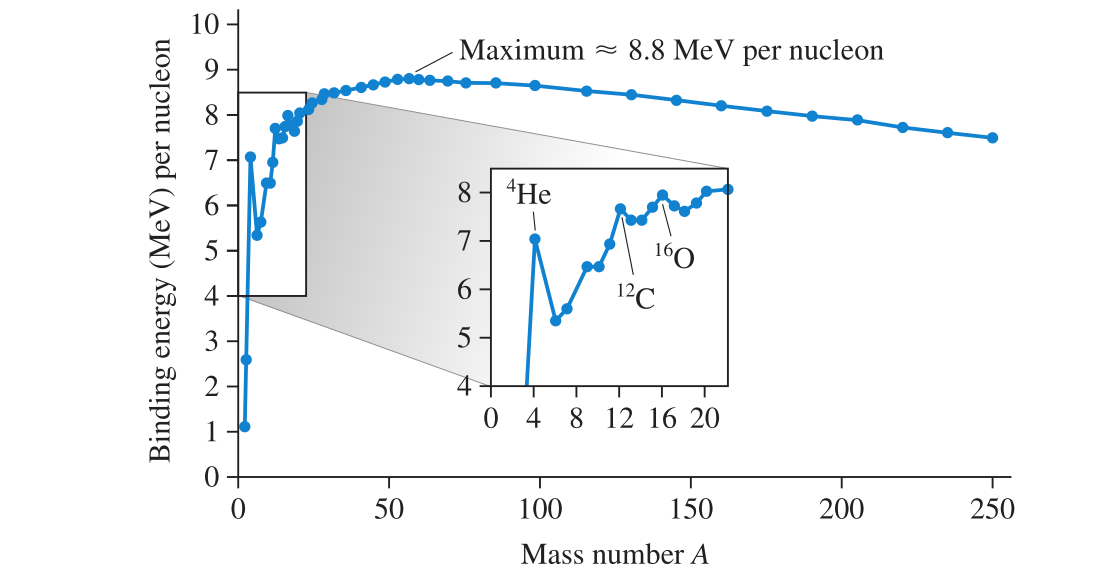
\includegraphics[scale=0.15]{fig_curve.png}
\end{center}
\end{topicbox}

\begin{topicbox}{Nuclear Forces}

\noindent Interactions within the nucleus are governed by two nuclear forces:
\begin{itemize}
\item The \emph{strong nuclear force}, which is an attractive force between any two nucleons.  It is a short-range force and is stronger than the electromagnetic force. 
\item The \emph{weak nuclear force} is involved in the process of beta decay, which turns a neutron into a proton, emitting an electron and antineutrino, as well as the reverse reaction.
\end{itemize}

\end{topicbox}

\begin{topicbox}{Radioactivity}

\noindent Many nuclei are unstable and decay to a different nucleus while emitting an alpha ($\alpha$), beta ($\beta$), or gamma ($\gamma$) ray. This is a random quantum mechanical process. The \emph{decay rate} $r$ is the probability that a particular nuclei will decay within the next second.  The number of nuclei $N$ in a sample will undergo exponential decay:
\begin{eqbox}
N = N_0 e^{-t/\tau},
\end{eqbox}
\noindent where $N_0$ is the number of nuclei at time $t = 0$ and $\tau = 1/r$ is the \emph{lifetime} of the nucleus.

More commonly is the half-life $t_{1/2}$, which is the time in which half of a sample of radioactive atoms decays:
\begin{eqbox}
N = N_0 \left( \frac{1}{2} \right)^{t/t_{1/2}}.
\end{eqbox}
\noindent The lifetime and half-life are related by $t_{1/2} = \tau \ln 2$.


The \emph{activity} $R$ of a radioactive sample is the number of decays per second:
\[
R = \left| \frac{dN}{dt} \right| = R_0 \left( \frac{1}{2} \right)^{t/t_{1/2}},
\]
\noindent where $R_0 = rN_0$ is the activity at $t=0$.  The SI unit of activity is the becquerel (1 Bq = 1 decay/s), although curies are also popular:
\[
1 \text{ Ci} = 3.7 \times 10^{10} \text{ Bq}.
\]
\vspace{0.1in}

\noindent \textbf{Alpha Decay}

\noindent A heavy parent nucleus X can decay to a lighter daughter nucleus Y by emitting an alpha particle (a $^4$He nucleus):
\begin{eqbox}
^A\text{X}_Z \to \, ^{A-4}\text{Y}_{Z-2} + \alpha + \text{energy}.
\end{eqbox}
\noindent The energy goes almost entirely into the kinetic energy of the alpha particle:
\[
K_\alpha = (m_\text{X} - m_\text{Y} - m_\text{He} ) c^2.
\]

\vspace{0.1in}

\noindent \textbf{Beta Decay}

\noindent Nuclei with too many protons or neutrons can undergo beta decay to move closer to the \emph{line of stability}.  The decay can emit an electron (beta-minus decay) or a positron (beta-plus decay):
\begin{eqbox}
^A\text{X}_Z \to \, ^{A}\text{Y}_{Z+1} + \text{e}^- + \text{energy}, \quad ^A\text{X}_Z \to \, ^{A}\text{Y}_{Z-1} + \text{e}^+ + \text{energy}
\end{eqbox}


\vspace{0.1in}


\noindent \textbf{Gamma Decay}

\noindent Gamma decay occurs when a nucleus makes a quantum transition from an excited energy state to a lower-energy state by emitting a high-energy photon. Alpha and beta decay often leave the daughter nucleus in an excited state, so gamma emission is usually found to accompany those decays.

\end{topicbox}






\end{multicols}

\makebanner{Electricity and Magnetism}

\end{document}



